\chapter{Obrada audio signala}

Nakon otvaranja audio datoteke, vrši se obrada zvučnog signala. Audio biblioteka \textit{SoundFile} koristi se za učitavanje audio datoteke te, pozivom \lstinline|sf.read(file_path)| dobivaju se matrica amplituda i frekvencija uzorkovanja. Dobivena matrica reprezentacija je audio signala u vremenskoj domeni, odnosno prikazuje glasnoću (amplitudu) zvuka dok se mijenja u vremenu. Amplituda jednaka nuli označava tišinu.

Za analizu odnosa amplitude i frekvencije signala potrebno transformirati signal u frekvencijsku domenu kako bi se prikazalo koje frekvencije se nalaze u signalu. Fourierovom transformacijom signal se dekomponira u odgovarajuće frekvencije. \textit{Scipy} biblioteka sadrži ugrađenu funkciju za brzu Fourierovu transformaciju.

Dobivene matrice iscrtavaju se grafički pomoću biblioteke \textit{matplotlib}. Ograničen je prikaz frekvencija na 2000 Hz...


\begin{figure}[ht]
	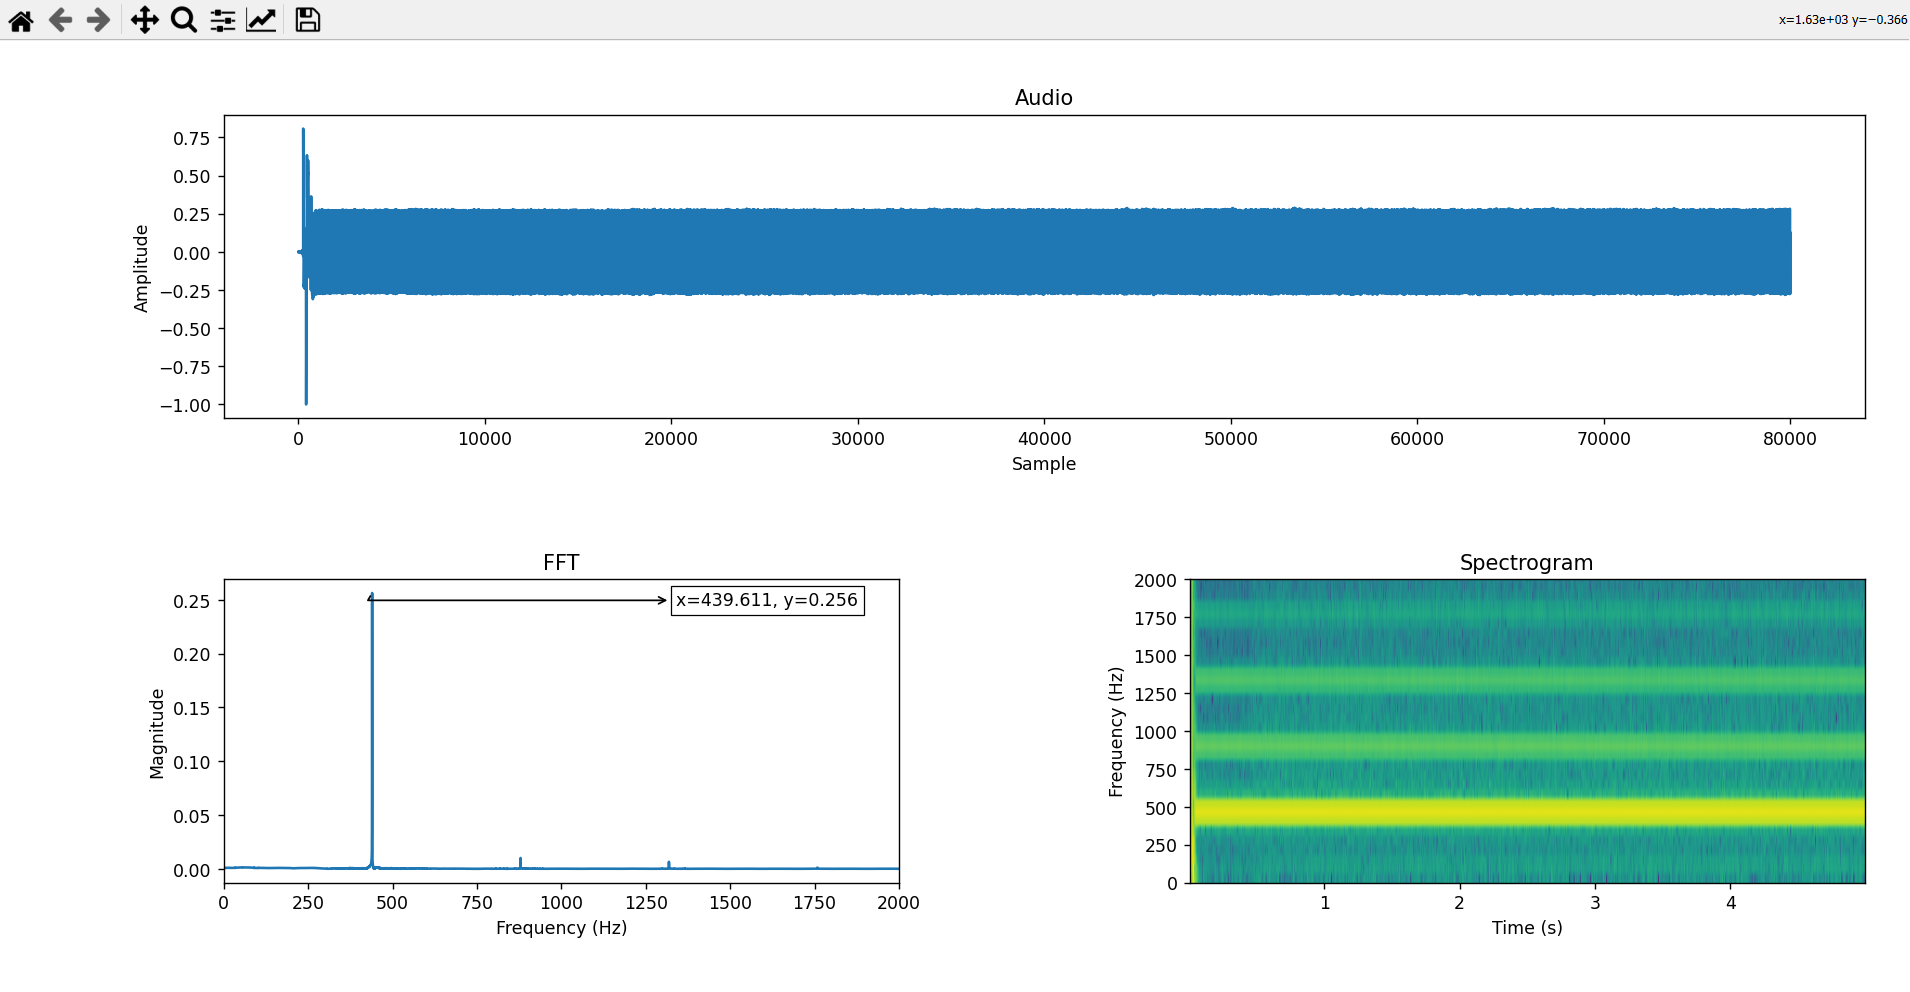
\includegraphics[width=\linewidth]{imgs/analyse_example}
	\caption{Primjer prikaza analize audiozapisa}
	\label{fig:analyse_example}
\end{figure}
